%! TeX program = xelatex

\documentclass[12pt, a4paper]{article}
\usepackage{cmap}
\usepackage[fontsize=12pt]{scrextend}
\usepackage[T2A]{fontenc}
\usepackage[utf8]{inputenc}
\usepackage[english,russian]{babel}
\usepackage{amsmath,amsfonts,amssymb,amsthm,mathtools}
\usepackage[left=20mm, top=20mm, right=20mm, bottom=20mm, nohead, footskip=1cm]{geometry}
\usepackage{multirow}
\usepackage{array}
\usepackage{multicol}
\usepackage{graphicx}
\usepackage{wrapfig}
\usepackage{indentfirst}
\usepackage{enumitem}

\usepackage{polyglossia}
\usepackage{titlesec}
\usepackage{sectsty}
\usepackage{setspace}
\usepackage{fontspec}
\defaultfontfeatures{Mapping=tex-text}

\usepackage{lipsum}
\usepackage{tocloft}
\usepackage[dvipsnames]{xcolor}

\usepackage{caption}
%\captionsetup{labelfont=it, textfont=it}
%\captionsetup[figure]{name=Схема}

\usepackage{hyperref}

\hypersetup{
    colorlinks=false,
    linktoc=all
}
\urlstyle{same}

\setmainlanguage{english}
\setotherlanguage{russian}
\setkeys{russian}{babelshorthands=true}
\setmainfont{Times New Roman}
\newfontfamily\cyrillicfont{Times New Roman}
%\let\cyrillicfonttt\ttfamily
%\onehalfspacing

%\allsectionsfont{\centering}
\renewcommand{\cftsecleader}{\cftdotfill{\cftdotsep}}

%======================================SECTIONING=========================================
%\makeatletter
%\renewcommand*\l@section{\@dottedtocline{1}{1.5em}{2.3em}}
%\makeatother
%======================================SECTIONING=========================================

\pretolerance=6000
\tolerance=3000
\emergencystretch=4pt

\setlength\intextsep{10pt}

\graphicspath{{./visuals/}}
\setlength{\parskip}{0.3125cm}
\setlength{\parindent}{1.25cm}
\setlength{\columnsep}{1cm}
\author{Grigoryev Mikhail}
\title{Algs lab}

\begin{document}

\thispagestyle{empty}

\vspace{30mm}

\begin{center}
FEDERAL STATE AUTONOMOUS EDUCATIONAL INSTITUTION \\
OF HIGHER EDUCATION \\
ITMO UNIVERSITY

\vspace{40mm}

{\large \textbf{Report \\
on the practical task No. 6 \\
"Algorithms on graphs. Path search algorithms on weighted graphs"}}
\end{center}

\vspace{15mm}

\begin{flushright}
{\large Performed by \\
\textit{Mikhail Grigoryev (370852) \\
Semenova Valeria (370061) \\
Academic group J4133c \\}
Accepted by \\
Dr Petr Chunaev}
\end{flushright}

\vspace{80mm}

\begin{center}
St. Petersburg \\
2022
\end{center}

\newpage

\section*{Goal}
\addcontentsline{toc}{section}{Goal}

The use of path search algorithms on weighted graphs (Dijkstra's, A* and Bellman-Ford algorithms).

\section*{Formulation of the problem}
\addcontentsline{toc}{section}{Formulation of the problem}

\textbf{Task 1.} Generate a random adjacency matrix for a simple undirected weighted graph of 100 vertices and 500 edges with assigned random positive integer weights (note that the matrix should be symmetric and contain only 0s and weights as elements). Use Dijkstra's and Bellman-Ford algorithms to find shortest paths between a random starting vertex and other vertices. Measure the time required to find the paths for each algorithm. Repeat the experiment 10 times for the same starting vertex and calculate the average time required for the paths search of each algorithm. Analyse the results obtained.

\textbf{Task 2.} Generate a 10$\times$20 cell grid with 40 obstacle cells. Choose two random non-obstacle cells and find a shortest path between them using A* algorithm. Repeat the experiment 5 times with different random pair of cells. Analyse the results obtained.

\section*{Brief theoretical part}
\addcontentsline{toc}{section}{Brief theoretical part}

Path search algorithms on graphs are used to find shortest paths between two vertices. In case of unweighted graphs, those paths consist of the least number of edges. In this practical work, however, graphs are weighted which means that numbers (costs) are assigned to the edges. Here, the shortest path between two vertices is defined as the path with the least sum of edge costs.

Algorithms used in this practical work (implemented from NetworkX library):
\begin{enumerate}
	\item Dijkstra's algorithm -- a search algorithm for weighted graphs with positive costs only. The algorithm uses tentative distances of vertices of the graph (lengths of shortest paths between the starting node and the current one). At each step, all neighbors of the current vertex are taken into account. Their tentative distances are measured, and, if better than previous values, are updated (paths are logged). When the current node is the end node, tentative distance is updated and the shortest logged path is taken as the shortest one.
	\item Bellman-Ford algorithm (although slower than Dijkstra's) can be used even on weighted graphs with negative costs. The algorithm initializes all nodes with infinite distances and then for all edges updates the distances to lower values if taking that edge lowers the distance to the destination. As the longest possible path (with no cycles) is $|V| - 1$ edges long, the edges must be scanned that many times to make sure that all of the paths to the nodes were optimized. This algorithm can detect negative loops (loops with costs adding up to a negative value) as in those cases no shortest path exists.
	\item A* algorithm is complete and extremely fast but requires vast amounts of additional memory.It utilizes heuristics in a sense that at every iteration it estimates which paths have to be extended (based on the cost of the path to the current node plus heuristic function that estimates the cheapest path from the node to the goal). The algorithm terminates when the extended path is the one from the start to the goal or when there are no paths to be extended.
\end{enumerate}

\newpage

\section*{Results}
\addcontentsline{toc}{section}{Results}

\textbf{Task 1.} A random adjacency matrix for a simple undirected weighted graph of 100 vertices and 500 edges was generated. The edge costs were chosen randomly as integers from 1 to 20. The starting vertex from the graph was chosen randomly, then Dijkstra's and Bellman-Ford algorithms were applied to find the shortest (in terms of costs) path between the starting and all other vertices. The computation was repeated 9 more times and the runtimes were measured and averaged.

Presented below is an example path between the starting node (50) and the current target (61). The path consists of 6 edges and 7 vertices:
\[ 50 \xrightarrow{3} 64 \xrightarrow{1} 33 \xrightarrow{1} 84 \xrightarrow{1} 25 \xrightarrow{1} 52 \xrightarrow{2} 61 \]
however, their costs add up to only 9.
\begin{figure}[!h]
	\centering
	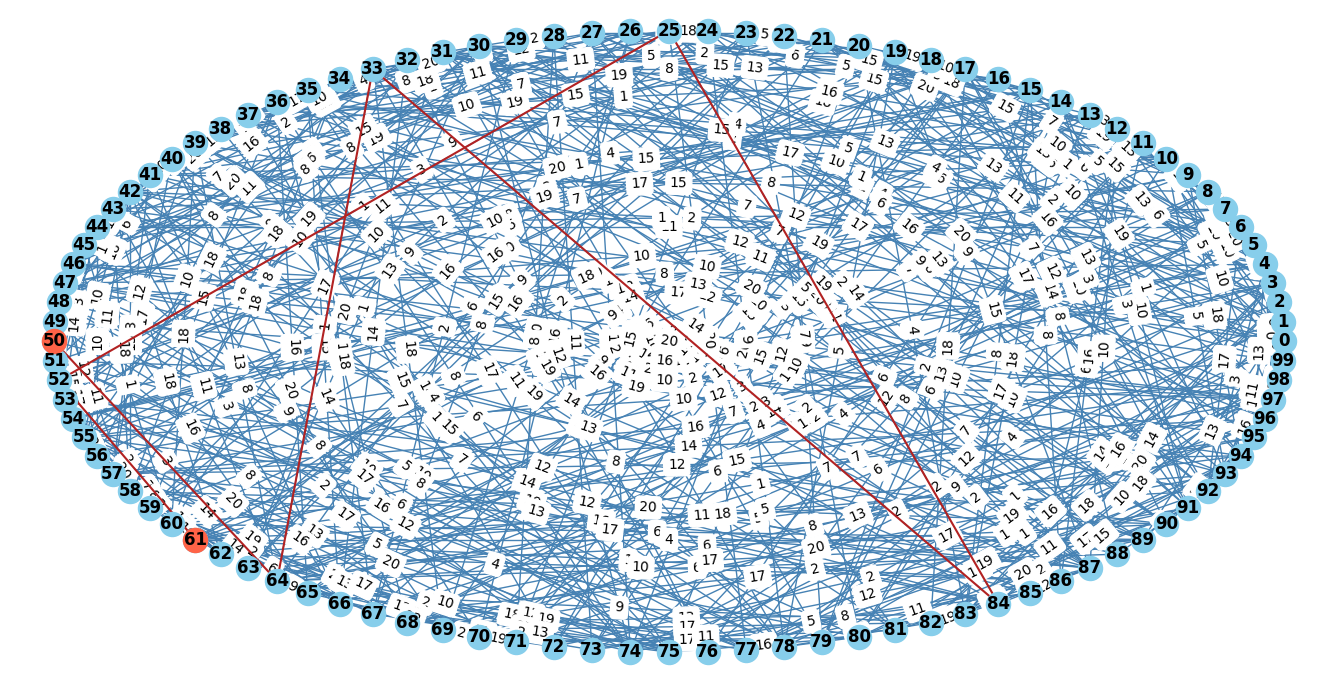
\includegraphics[width=\textwidth]{task1.png}
	\caption{Example of a shortest path between two random vertices. Here the path consists of many edges, however, the costs of each are low.}
\end{figure}

In the task, shortest paths were computed from a randomly selected vertex to all other vertices in the graph by means of Dijkstra's and Bellman-Ford algorithms. Results for the starting vertex 50:
\[ \begin{matrix} \text{Dijkstra:} & 0.0162 \text{ s} \\
\text{Bellman-Ford:} & 0.0607 \text{ s} \end{matrix} \] 

The results prove that Dijkstra's algorithm significantly faster than Bellman-Ford. The latter has an added benefit of working on weighted graphs with negative costs which was not covered in the present work.

\newpage

\textbf{Task 2.} The random 10$\times$20 grid with 40 obstacle cells was represented by a graph, where each cell is a node and edges exist only between adjacent cells in the grid. Obstacle cells were represented by the lack of vertex in its place. Two random non-obstacle cells were chosen and the shortest path between them was computed via A* algorithm. Such computations for different random pairs were executed five times. The computation runtimes were measured and presented on the graph below.
\begin{figure}[!h]
	\centering
	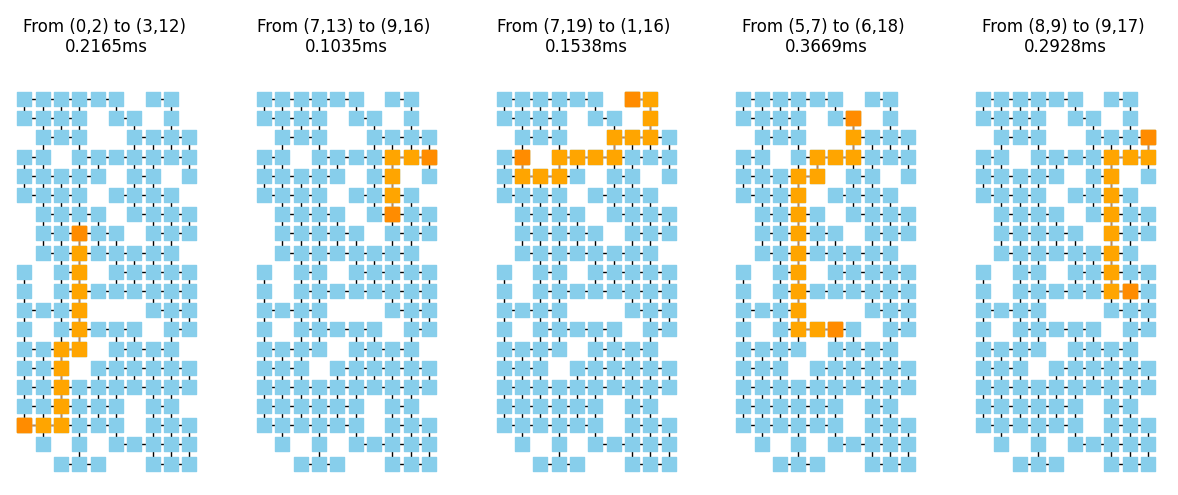
\includegraphics[width=\textwidth]{task2.png}
	\caption{Five shortest paths (A*) in a random 10$\times$20 grid with 40 obstacles with execution times.}
\end{figure}

According to the obtained data, the execution time is correlated with the length of the shortest path. The further the cells are located, the longer the algorithm runs in search of it.

\section*{Conclusions}
\addcontentsline{toc}{section}{Conclusions}

Path search algorithms for weighted graphs such as Dijkstra's, Bellman-Ford and A* algorithms were applied for searching the shortest path between random vertices in random graphs, both weighted and unweighted. The former two algorithms were compared in performance.

\section*{Appendix}
\addcontentsline{toc}{section}{Appendix}

GitHub link (task 1): \url{https://github.com/Dormant512/itmo_lab_listings/blob/main/lab6_1.py}.

GitHub link (task 2): \url{https://github.com/Dormant512/itmo_lab_listings/blob/main/lab6_2.py}.

\begin{figure}[!h]
\centering

\includegraphics[width=0.25\textwidth]{lab6-1.png}

\includegraphics[width=0.25\textwidth]{lab6-2.png}
\end{figure}


\end{document}
